\documentclass[12pt]{article}
\usepackage{amsmath}
\usepackage{latexsym}
\usepackage{amsfonts}
\usepackage[normalem]{ulem}
\usepackage{array}
\usepackage{amssymb}
\usepackage{graphicx}
\usepackage[backend=biber,
style=numeric,
sorting=none,
isbn=false,
doi=false,
url=false,
]{biblatex}\addbibresource{bibliography.bib}

\usepackage{subfig}
\usepackage{wrapfig}
\usepackage{wasysym}
\usepackage{enumitem}
\usepackage{adjustbox}
\usepackage{ragged2e}
\usepackage[svgnames,table]{xcolor}
\usepackage{tikz}
\usepackage{longtable}
\usepackage{changepage}
\usepackage{setspace}
\usepackage{hhline}
\usepackage{multicol}
\usepackage{tabto}
\usepackage{float}
\usepackage{multirow}
\usepackage{makecell}
\usepackage{fancyhdr}
\usepackage[toc,page]{appendix}
\usepackage[hidelinks]{hyperref}
\usetikzlibrary{shapes.symbols,shapes.geometric,shadows,arrows.meta}
\tikzset{>={Latex[width=1.5mm,length=2mm]}}
\usepackage{flowchart}\usepackage[paperheight=11.0in,paperwidth=8.5in,left=1.0in,right=1.0in,top=1.0in,bottom=1.0in,headheight=1in]{geometry}
\usepackage[utf8]{inputenc}
\usepackage[T1]{fontenc}
\TabPositions{0.5in,1.0in,1.5in,2.0in,2.5in,3.0in,3.5in,4.0in,4.5in,5.0in,5.5in,6.0in,}

\urlstyle{same}


 %%%%%%%%%%%%  Set Depths for Sections  %%%%%%%%%%%%%%

% 1) Section
% 1.1) SubSection
% 1.1.1) SubSubSection
% 1.1.1.1) Paragraph
% 1.1.1.1.1) Subparagraph


\setcounter{tocdepth}{5}
\setcounter{secnumdepth}{5}


 %%%%%%%%%%%%  Set Depths for Nested Lists created by \begin{enumerate}  %%%%%%%%%%%%%%


\setlistdepth{9}
\renewlist{enumerate}{enumerate}{9}
		\setlist[enumerate,1]{label=\arabic*)}
		\setlist[enumerate,2]{label=\alph*)}
		\setlist[enumerate,3]{label=(\roman*)}
		\setlist[enumerate,4]{label=(\arabic*)}
		\setlist[enumerate,5]{label=(\Alph*)}
		\setlist[enumerate,6]{label=(\Roman*)}
		\setlist[enumerate,7]{label=\arabic*}
		\setlist[enumerate,8]{label=\alph*}
		\setlist[enumerate,9]{label=\roman*}

\renewlist{itemize}{itemize}{9}
		\setlist[itemize]{label=$\cdot$}
		\setlist[itemize,1]{label=\textbullet}
		\setlist[itemize,2]{label=$\circ$}
		\setlist[itemize,3]{label=$\ast$}
		\setlist[itemize,4]{label=$\dagger$}
		\setlist[itemize,5]{label=$\triangleright$}
		\setlist[itemize,6]{label=$\bigstar$}
		\setlist[itemize,7]{label=$\blacklozenge$}
		\setlist[itemize,8]{label=$\prime$}

\setlength{\topsep}{0pt}\setlength{\parskip}{8.04pt}
\setlength{\parindent}{0pt}

 %%%%%%%%%%%%  This sets linespacing (verticle gap between Lines) Default=1 %%%%%%%%%%%%%%


\renewcommand{\arraystretch}{1.3}


%%%%%%%%%%%%%%%%%%%% Document code starts here %%%%%%%%%%%%%%%%%%%%



\begin{document}

\vspace{\baselineskip}
\begin{Center}
{\fontsize{16pt}{19.2pt}\selectfont \textbf{SOEN 6481}\par}
\end{Center}\par


\vspace{\baselineskip}
\begin{Center}
{\fontsize{16pt}{19.2pt}\selectfont \textbf{Software Requirement Specification}\par}
\end{Center}\par


\vspace{\baselineskip}
\begin{Center}
{\fontsize{16pt}{19.2pt}\selectfont \textbf{Summer 2019}\par}
\end{Center}\par


\vspace{\baselineskip}
\begin{Center}
{\fontsize{16pt}{19.2pt}\selectfont \textbf{Deliverable 1}\par}
\end{Center}\par


\vspace{\baselineskip}
\begin{Center}
{\fontsize{16pt}{19.2pt}\selectfont \textbf{Eternity: Numbers}\par}
\end{Center}\par


\vspace{\baselineskip}
\begin{Center}
{\fontsize{16pt}{19.2pt}\selectfont \textbf{Declaration}\par}
\end{Center}\par


\vspace{\baselineskip}
\begin{justify}
{\fontsize{16pt}{19.2pt}\selectfont \textbf{I have read and understood the Fairness Protocol and Communal Work Protocol, and agree to abide by the policies therein, without any exception under any circumstances, whatsoever.}\par}
\end{justify}\par


\vspace{\baselineskip}
\begin{justify}
{\fontsize{16pt}{19.2pt}\selectfont \textbf{\ \ \ \ \ \ \ \ \ \ \ \ \ \ \ \ \ \ \ \ \ \ \ \ \ \ \ \ \ \ \ \ \ \ \ \ \ \ \ \  By: Sargun Kaur Dhanju}\par}
\end{justify}\par

\begin{justify}
{\fontsize{16pt}{19.2pt}\selectfont \textbf{\ \ \ \ \ \ \ \ \ \ \ \ \ \ \ \ \ \ \ \ \ \ \ \ \ \ \ \ \ \ \ \ \ \ \ \ \ \ \ \ \ \ \ \ \ \ \ \ \ \  (40071167)}\par}
\end{justify}\par


\vspace{\baselineskip}

\vspace{\baselineskip}

\vspace{\baselineskip}

\vspace{\baselineskip}

\vspace{\baselineskip}

\vspace{\baselineskip}

\vspace{\baselineskip}

\vspace{\baselineskip}

\vspace{\baselineskip}

\vspace{\baselineskip}

\vspace{\baselineskip}

\vspace{\baselineskip}

\vspace{\baselineskip}

\vspace{\baselineskip}

\vspace{\baselineskip}
\begin{justify}
{\fontsize{14pt}{16.8pt}\selectfont \textbf{Table of Contents}\par}
\end{justify}\par

\begin{enumerate}
	\item Problem 1$ \ldots $ $ \ldots $ $ \ldots $ $ \ldots $ $ \ldots $ $ \ldots $ $ \ldots $ $ \ldots $ $ \ldots $ $ \ldots $ $ \ldots $ $ \ldots $ $ \ldots $ $ \ldots $ $ \ldots $ $ \ldots $ ...3\par

	\item Problem 2$ \ldots $ $ \ldots $ $ \ldots $ $ \ldots $ $ \ldots $ $ \ldots $ $ \ldots $ $ \ldots $ $ \ldots $ $ \ldots $ $ \ldots $ $ \ldots $ $ \ldots $ $ \ldots $ $ \ldots $ $ \ldots $ ...4\par

	\item Problem 3$ \ldots $ $ \ldots $ $ \ldots $ $ \ldots $ $ \ldots $ $ \ldots $ $ \ldots $ $ \ldots $ $ \ldots $ $ \ldots $ $ \ldots $ $ \ldots $ $ \ldots $ $ \ldots $ $ \ldots $ $ \ldots $ ...6\par

	\item Problem 4$ \ldots $ $ \ldots $ $ \ldots $ $ \ldots $ $ \ldots $ $ \ldots $ $ \ldots $ $ \ldots $ $ \ldots $ $ \ldots $ $ \ldots $ $ \ldots $ $ \ldots $ $ \ldots $ $ \ldots $ $ \ldots $ ...7\par

	\item Problem 5$ \ldots $ $ \ldots $ $ \ldots $ $ \ldots $ $ \ldots $ $ \ldots $ $ \ldots $ $ \ldots $ $ \ldots $ $ \ldots $ $ \ldots $ $ \ldots $ $ \ldots $ $ \ldots $ $ \ldots $ $ \ldots $ ...8\par

	\item Glossary$ \ldots $ $ \ldots $ $ \ldots $ $ \ldots $ $ \ldots $ $ \ldots $ $ \ldots $ $ \ldots $ $ \ldots $ $ \ldots $ $ \ldots $ $ \ldots $ $ \ldots $ $ \ldots $ $ \ldots $ $ \ldots $ $ \ldots $ 11\par

	\item References$ \ldots $ $ \ldots $ $ \ldots $ $ \ldots $ $ \ldots $ $ \ldots $ $ \ldots $ $ \ldots $ $ \ldots $ $ \ldots $ $ \ldots $ $ \ldots $ $ \ldots $ $ \ldots $ $ \ldots $ $ \ldots $ 11
\end{enumerate}\par


\vspace{\baselineskip}

\vspace{\baselineskip}

\vspace{\baselineskip}

\vspace{\baselineskip}

\vspace{\baselineskip}

\vspace{\baselineskip}

\vspace{\baselineskip}

\vspace{\baselineskip}

\vspace{\baselineskip}

\vspace{\baselineskip}

\vspace{\baselineskip}

\vspace{\baselineskip}

\vspace{\baselineskip}

\vspace{\baselineskip}

\vspace{\baselineskip}

\vspace{\baselineskip}

\vspace{\baselineskip}

\vspace{\baselineskip}

\vspace{\baselineskip}

\vspace{\baselineskip}

\vspace{\baselineskip}

\vspace{\baselineskip}

\vspace{\baselineskip}

\vspace{\baselineskip}

\vspace{\baselineskip}

\vspace{\baselineskip}

\vspace{\baselineskip}

\vspace{\baselineskip}

\vspace{\baselineskip}

\vspace{\baselineskip}

\vspace{\baselineskip}

\vspace{\baselineskip}

\vspace{\baselineskip}

\vspace{\baselineskip}

\vspace{\baselineskip}

\vspace{\baselineskip}
\begin{Center}
{\fontsize{14pt}{16.8pt}\selectfont \textbf{Pi ($ \pi $ )}\par}
\end{Center}\par

\begin{justify}
{\fontsize{14pt}{16.8pt}\selectfont \textbf{Problem 1. [20 Marks]}\par}
\end{justify}\par

\begin{justify}
\href{https://www.wonderopolis.org/wonder/what-is-pi}{Pi} (represented as  $ \pi $ ) is the ratio of a circle's \href{https://www.wonderopolis.org/wonder/what-is-pi}{circumference} to its \href{https://www.wonderopolis.org/wonder/what-is-pi}{diameter}. The value of $ \pi $  remains same regardless of the size of the circle. So, for any circle, dividing its \href{https://www.wonderopolis.org/wonder/what-is-pi}{circumference} by its \href{https://www.wonderopolis.org/wonder/what-is-pi}{diameter} will give us the exact same value i.e. 3.14159$ \ldots $  Being an irrational number, it never ends and its value cannot be represented as a simple fraction. Although 22/7 is used generally that gives the result that is close to $ \pi $  [1].  Most calculators have a button to enter the value of $ \pi $  directly. Using $ \pi $  button in the calculator is better, because it inputs it to the greatest number of decimal places that the calculator is capable of.
\end{justify}\par

\begin{justify}
It plays a very prominent role in the area of mathematics. $ \Pi $  appears in formula for areas and volumes of many geometrical shapes based on circles such as spheres, cones etc. Trigonometric functions rely on angles and angles are measured in radians. A complete circle spans an angle of 2 $ \pi $ . It is also used in Cauchy’s distribution which is a probability density function. Other than these, $ \pi $  is used in Fourier Series, Gaussian Integrals, Topology, Vector Calculus etc [1].
\end{justify}\par

\begin{justify}
Apart from mathematics, $ \pi $  can be used in other natural phenomena. It can measure things like ocean waves, light waves, sound waves, river bends, radioactive particle distribution etc.
\end{justify}\par

\begin{justify}
\textbf{Other applications of pi-}
\end{justify}\par

\begin{itemize}
	\item Electrical engineers use $ \pi $  to solve problems for electrical applications.\par

	\item Statisticians use it for tracking population dynamics. \par

	\item Medicine benefits from $ \pi $  when studying structure of the eye.\par

	\item Clock designers use it for designing pendulums for clocks.\par

	\item Aircraft designers use it for calculating areas of the skin of the aircraft [2].
\end{itemize}\par


\vspace{\baselineskip}
\begin{justify}
\textbf{Some of the characteristics that make $ \pi $  unique from other irrational numbers-}
\end{justify}\par

\begin{justify}
An interesting thing about $ \pi $  is that there are no repeating patterns in digits of it. It is transcendental and not algebraic. $ \Pi $  is special because it describes the geometry of circles. Any statement about $ \pi $  that has substance relates it to the circle, and to prove irrationality, transcendentalism and normality, we have to relate $ \pi $  to the circle in a way that gives us these results [3].  The beauty of $ \pi $ , in part, is that it puts infinity within reach. $ \pi $  touches infinity in other ways. For example, there are astonishing formulas in which an endless procession of smaller and smaller numbers adds up to $ \pi $ . One of the earliest such infinite series to be discovered says that $ \pi $  equals four times the sum 1 – \textsuperscript{1}⁄\textsubscript{3} + \textsuperscript{1}⁄\textsubscript{5} – \textsuperscript{1}⁄\textsubscript{7} + \textsuperscript{1}⁄\textsubscript{9} – \textsuperscript{1}⁄\textsubscript{11} + $ \cdots $ . It connects all odd numbers to $ \pi $ , thereby also linking number theory to circles and geometry. In this way, $ \pi $  joins two seemingly separate mathematical universes [4]. Its ubiquity goes beyond mathematics. This number crops up in the real world too [5].
\end{justify}\par


\vspace{\baselineskip}

\vspace{\baselineskip}
\begin{justify}
{\fontsize{14pt}{16.8pt}\selectfont \textbf{Problem 2. [20 Marks]}\par}
\end{justify}\par

\begin{justify}
Interviewer (Sargun): Hi Sonal, I am working on a project called Eternity: Numbers which focuses on different irrational numbers. I am specifically working on the number $``$$ \pi $ $"$ .\  So, can I ask you some questions about it?
\end{justify}\par

\begin{justify}
Interviewee (Sonal): Of course.
\end{justify}\par

\begin{justify}
Sargun: Sonal what do you do?
\end{justify}\par

\begin{justify}
Sonal: I am a Senior Scientist in Siemens, Germany working in the field of medical imaging. I did my PhD in Engineering and Postdoctoral work in Radiology at Stanford University with a research focus in development of new and advanced techniques for magnetic resonance imaging (MRI).
\end{justify}\par

\begin{justify}
Sargun: Impressive! So how often do you use irrational numbers, or $ \pi $  in specific, in your work? 
\end{justify}\par

\begin{justify}
Sonal: We use many formulae in our work, and most of them use irrational numbers. Among them, $``$$ \pi $ $"$  and $``$e$"$  occurs most of the time. Whenever we are working on something, and we have circles, we always encounter $ \pi $ . I also had a subject in my degree that dealt with mathematics and physics and I have worked with $ \pi $  in the projects associated with that course. 
\end{justify}\par

\begin{justify}
Sargun: Okay. Which is your favourite irrational number?
\end{justify}\par

\begin{justify}
Sonal: Well I think you have found the right person for your interview because my favourite irrational number is $``$$ \pi $ $"$ .
\end{justify}\par

\begin{justify}
Sargun: Perfect! Do you use a calculator that provides you with the values of irrational numbers that you use in your work?
\end{justify}\par

\begin{justify}
Sonal: We use it, but not always. If I talk about my current work place, I have a chart there which displays the values of all the famous and frequently used irrational numbers.
\end{justify}\par

\begin{justify}
Sargun: Okay. Can you tell me a few interesting facts about $ \pi $ ?
\end{justify}\par

\begin{justify}
Sonal: When I was in U.S, I went to attend $ \pi $  day celebration once. It takes place on March 14 in San Francisco. It is celebrated on this day as March is the third month of the year, so it is 3/14. Another interesting fact is that digits of $ \pi $  can never be fully known. In earlier times, people used to find out the value of $ \pi $  to up to 1000 places. Imagine doing this by hand with no calculators. This has become a thing of the past, since the monotony that was done by hand is now done by computer.
\end{justify}\par

\begin{justify}
Sargun: Alright. Why is $ \pi $  so important?
\end{justify}\par

\begin{justify}
Sonal: $ \pi $  is important because it is related to cycles. When we apply mathematics to the real world, it makes $ \pi $  absolutely necessary. There is a major formula in mathematics called Fourier Series whose building blocks are $ \pi $ . $ \pi $  is also used in designing of buildings to withstand earthquakes. We can say that cycles are temporal cousins of circles, so $ \pi $  will occur every time we are working with circles. 
\end{justify}\par


\vspace{\baselineskip}
\begin{justify}
Sargun: Why is $ \pi $  defined as a ratio of two rational numbers if it is an irrational number?
\end{justify}\par

\begin{justify}
Sonal: This is an interesting question! $ \Pi $  is the ratio of diameter and circumference of the circle and these two will never be rational numbers. When we measure them, we get their approximate values and we can take their ratio to find the approximation of $ \pi $ .
\end{justify}\par

\begin{justify}
Sargun: But how is that possible? If I draw a circle, I can measure its diameter. How can this measurement be irrational?
\end{justify}\par

\begin{justify}
Sonal: Good observation! But one of them, either the circumference or the diameter is irrational. The diameter of the circle that you measured, no matter how accurately you measured it, it will never be accurate enough and same goes for the circumference. It will be an irrational value. You can never know the diameter or circumference exactly just by measuring it.
\end{justify}\par

\begin{justify}
Sargun: Oh, I see! I have to design a calculator that makes calculations using $ \pi $ . Can you suggest me that for what all parameters can I use it?
\end{justify}\par

\begin{justify}
Sonal:\tab That sounds fun. You can use it for any of the basic formulas of circles, like calculating the area, circumference, length of circle’s arc, etc and you can calculate same things for the cylinders too. You can also calculate Fourier series with it!
\end{justify}\par

\begin{justify}
Sargun: Okay. That’s all! thank you so much for your time Sonal! It was a pleasure talking to you.
\end{justify}\par

\begin{justify}
Sonal: No problem. All the best for your project!
\end{justify}\par


\vspace{\baselineskip}
\begin{justify}
\textbf{Analysis of the interview-}
\end{justify}\par

\begin{justify}
Based on the interview, it can be analysed that the interviewee has encountered $ \pi $  and e most of the times. According to her, $ \pi $  is one of the most commonly occurring irrational numbers. In the field of mathematics and physics, $ \pi $  is used in all the formulas of circles. Among all the irrational numbers, she likes $ \pi $  the most. For the values of irrational numbers, she does not use a calculator as she has a chart at her work place that displays the values of irrational numbers. She explained the importance of $ \pi $  and illustrated its use in real world applications. She told that $ \pi $  will be used every time circles are involved. Some of the major formulas of mathematics are created by the use of $ \pi $ . She highlighted that while calculating the value of $ \pi $ , no matter how accurately we measure the parameters Circumference and Diameter, one of them is always an irrational value and because of this $ \pi $  turns out to be an irrational number. She also suggested some formulas that I can use in my calculator such as area and circumference of the circle and cylinder, length of the circle’s arc and Fourier Series. The interview was an unstructured interview. The interview protocol was followed. I followed Funnel model of interview.
\end{justify}\par


\vspace{\baselineskip}

\vspace{\baselineskip}
\begin{justify}
{\fontsize{14pt}{16.8pt}\selectfont \textbf{Problem 3. [40 Marks]}\par}
\end{justify}\par



%%%%%%%%%%%%%%%%%%%% Table No: 1 starts here %%%%%%%%%%%%%%%%%%%%


\begin{table}[H]
 			\centering
\begin{tabular}{p{4.51in}p{1.54in}}
\hline
%row no:1
\multicolumn{1}{|p{4.51in}}{\textbf{Private Information} \par {\fontsize{14pt}{16.8pt}\selectfont \textbf{\ \ \ \ \ \ \ \ \ \ \ \ \ \ \ \ \ \ \ \ \ \ \ \ \ \ \ \ \ \ \ \ \ \ \ \ \ \ \ \ \ \ \ \ \ \ \ \ \ \ \ \ \ \ \ \ \ \ \ \ \ \ \ \ \ \ \ \ \ \ \ \ \ \ \ \ \ \ \ \ \ \ \ \ \ \ \ \ \ \ \ \ \ \ \ \ \ \ \ \ \  }} \par Dr. Sonal Josan is 38 years old. She works at Siemens as a Senior Scientist. She is single and currently resides in Munich, Germany. She has a keen interest in Mathematics and Physics. She likes to read novels and travel. } & 
\multicolumn{1}{|p{1.54in}|}{
	\begin{Center}
		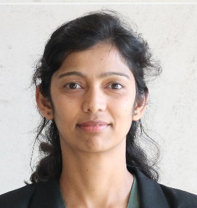
\includegraphics[width=1.54in,height=1.5in]{image1.png}
	\end{Center}
 \par } \\
\hhline{--}
%row no:2
\multicolumn{2}{|p{6.25in}|}{\textbf{Use of number, relation to Number} \par \begin{itemize}
	\item She has used $ \pi $  in her projects. \par 	\item She uses it whenever she has to use formulas related to circles in her work.
\end{itemize} \par } \\
\hhline{--}
%row no:3
\multicolumn{2}{|p{6.25in}|}{\textbf{Description of work or daily life} \par Dr. Sonal is working in the field of medical imaging. She did her PhD in Engineering and Postdoctoral work in Radiology at Stanford University with a research focus in development of new and advanced techniques for magnetic resonance imaging (MRI). Currently she is working with Siemens, and is continuing her research. \par } \\
\hhline{--}
%row no:4
\multicolumn{2}{|p{6.25in}|}{\textbf{Other uses or relations to the Number} \par She like $ \pi $  more than other irrational numbers. She had mathematical subjects in her degree in which she had worked with $ \pi $  in the projects of those subjects. \par } \\
\hhline{--}
%row no:5
\multicolumn{2}{|p{6.25in}|}{\textbf{Influencers that surround persona and that may influence choices} \par \begin{itemize}
	\item Colleagues at her workplace \par 	\item Her interest in Science \par 	\item Her research
\end{itemize} \par } \\
\hhline{--}

\end{tabular}
 \end{table}


%%%%%%%%%%%%%%%%%%%% Table No: 1 ends here %%%%%%%%%%%%%%%%%%%%


\vspace{\baselineskip}

\vspace{\baselineskip}

\vspace{\baselineskip}

\vspace{\baselineskip}

\vspace{\baselineskip}
\begin{justify}
{\fontsize{14pt}{16.8pt}\selectfont \textbf{Problem 4. [20 marks]}\par}
\end{justify}\par



%%%%%%%%%%%%%%%%%%%% Figure/Image No: 1 starts here %%%%%%%%%%%%%%%%%%%%

\begin{figure}[H]
	\begin{Center}
		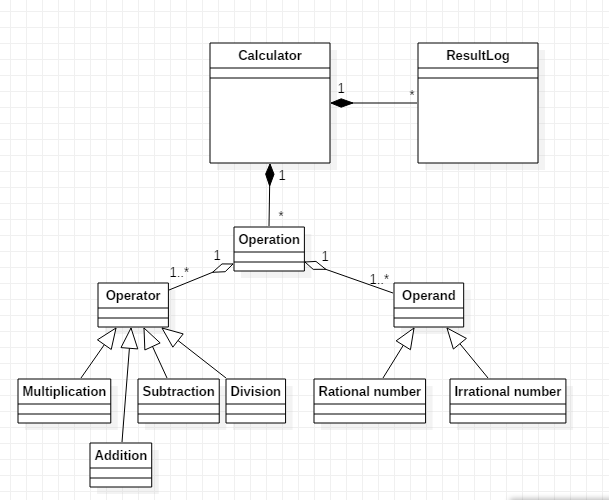
\includegraphics[width=6.55in,height=7.46in]{image2.png}
	\end{Center}
\end{figure}


%%%%%%%%%%%%%%%%%%%% Figure/Image No: 1 Ends here %%%%%%%%%%%%%%%%%%%%

\begin{justify}
 
\end{justify}\par

\begin{Center}
\textbf{Fig 1. $``$Problem Domain Model$"$ }
\end{Center}\par


\vspace{\baselineskip}

\vspace{\baselineskip}
\begin{justify}
{\fontsize{14pt}{16.8pt}\selectfont \textbf{Problem 5. [50 marks]}\par}
\end{justify}\par



%%%%%%%%%%%%%%%%%%%% Figure/Image No: 2 starts here %%%%%%%%%%%%%%%%%%%%

\begin{figure}[H]
	\begin{Center}
		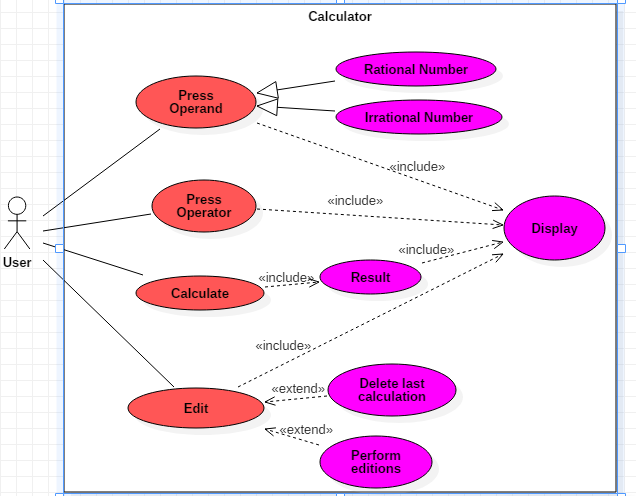
\includegraphics[width=6.61in,height=6.13in]{image3.png}
	\end{Center}
\end{figure}


%%%%%%%%%%%%%%%%%%%% Figure/Image No: 2 Ends here %%%%%%%%%%%%%%%%%%%%

\par

\begin{Center}
\textbf{Fig 2. $``$UML Use Case Diagram$"$ }
\end{Center}\par


\vspace{\baselineskip}

\vspace{\baselineskip}
\begin{enumerate}
	\item \textbf{Press Operand- }\par

\textbf{Pre-condition}- User has turned on the calculator.\par

\textbf{Main scenario}- User can use any kind of the operand i.e. rational number or irrational number to perform the computation.\par


\vspace{\baselineskip}

\vspace{\baselineskip}
	\item \textbf{Press Operator- }\par

\textbf{Pre-condition}- User has turned on the calculator and has entered an operand.\par

\textbf{Main scenario}- User can use any operator on the selected operands to perform the computation.\par

	\item \textbf{Calculate- }\par

\textbf{Pre-condition} User has selected the operands and operator.\par

\textbf{Main scenario}- User will perform the computation on the selected the operands and a result will be generated.\par

	\item \textbf{Edit- }\par

\textbf{Pre-condition} User has performed a computation.\par

\textbf{Main scenario}- If a user has made a mistake in performing the computation, or has entered a wrong operand or operator, the user can make the necessary editions or delete the last calculation.\par

	\item \textbf{Display- }
\end{enumerate}\par

\textbf{Pre-condition} User has entered something in the calculator.\par

\textbf{Main scenario}- Everything will be displayed, be it operand, operator, result or editions.\par


\vspace{\baselineskip}

\vspace{\baselineskip}

\vspace{\baselineskip}

\vspace{\baselineskip}

\vspace{\baselineskip}

\vspace{\baselineskip}

\vspace{\baselineskip}

\vspace{\baselineskip}

\vspace{\baselineskip}

\vspace{\baselineskip}

\vspace{\baselineskip}

\vspace{\baselineskip}

\vspace{\baselineskip}

\vspace{\baselineskip}

\vspace{\baselineskip}

\vspace{\baselineskip}

\vspace{\baselineskip}

\vspace{\baselineskip}

\vspace{\baselineskip}

\vspace{\baselineskip}

\vspace{\baselineskip}

\vspace{\baselineskip}

\vspace{\baselineskip}

\vspace{\baselineskip}

\vspace{\baselineskip}

\vspace{\baselineskip}

\vspace{\baselineskip}


%%%%%%%%%%%%%%%%%%%% Figure/Image No: 3 starts here %%%%%%%%%%%%%%%%%%%%

\begin{figure}[H]
	\begin{Center}
		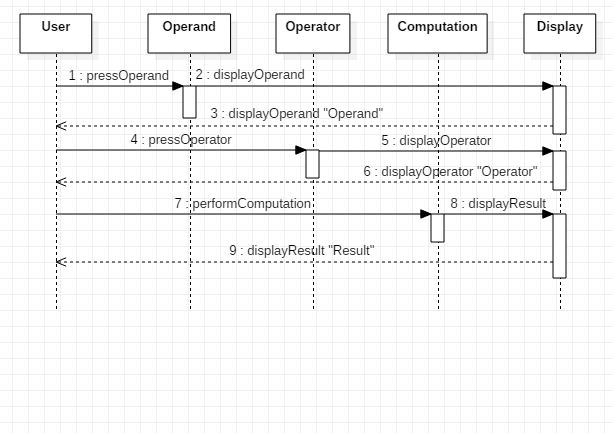
\includegraphics[width=6.34in,height=5.27in]{image4.png}
	\end{Center}
\end{figure}


%%%%%%%%%%%%%%%%%%%% Figure/Image No: 3 Ends here %%%%%%%%%%%%%%%%%%%%

\par

\begin{Center}
\textbf{Fig 3. $``$UML Sequence Diagram$"$ ’}
\end{Center}\par


\vspace{\baselineskip}
\begin{justify}
\textbf{Scenario to calculate circumference of a circle}
\end{justify}\par

\begin{enumerate}
	\item User will enter the operand $``$2$"$  and it will be displayed on the screen.\par

	\item User will enter the operator of $``$multiplication$"$  and it will be displayed on the screen.\par

	\item User will enter another operand $``$$ \pi $ $"$  and it will be displayed on the screen.\par

	\item The result will be displayed on the screen.\par

	\item User will enter the operator of $``$multiplication$"$  and another operand for the radius of the circle.\par

	\item The result will be displayed on the screen.
\end{enumerate}\par


\vspace{\baselineskip}

\vspace{\baselineskip}

\vspace{\baselineskip}
\begin{justify}
{\fontsize{14pt}{16.8pt}\selectfont \textbf{Glossary}\par}
\end{justify}\par

\begin{enumerate}
	\item Interview: a one-to-one conversation between an interviewer and an interviewee.\par

	\item Interviewer: a person who conducts an interview.\par

	\item Interviewee: a person who is interviewed.\par

	\item Persona: an aspect of someone’s character that is presented to or perceived by others.\par

	\item Use case: a specific situation in which a product could be used.
\end{enumerate}\par


\vspace{\baselineskip}
\begin{justify}
{\fontsize{14pt}{16.8pt}\selectfont \textbf{References}\par}
\end{justify}\par

{\fontsize{10pt}{12.0pt}\selectfont [1]\textbf{ }P. Kamthan, Summer 2019, $``$Project Description$"$ , Department of Computer Science and Software Engineering, Concordia University.\par}\par

{\fontsize{10pt}{12.0pt}\selectfont [2] Wikipedia, Pi, 2017 [Online]. \par}\par

{\fontsize{10pt}{12.0pt}\selectfont Available: \href{https://en.wikipedia.org/wiki/Pi#Role_and_characterizations_in_mathematics}{https://en.wikipedia.org/wiki/Pi$\#$ Role\_and\_characterizations\_in\_mathematics}\par}\par

{\fontsize{10pt}{12.0pt}\selectfont [3]\ Audrey, Adrian, Yu zheng and LeeWen. 2012. Amazing Discovery of Mathematics, Retrieved from:  \href{https://amazingarchimedes.weebly.com/real-life-application-of-pi.html}{https://amazingarchimedes.weebly.com/real-life-application-of-pi.html}\par}\par

{\fontsize{10pt}{12.0pt}\selectfont [4] Reddit, What makes Pi different from other irrational numbers, 2016 [Online]. \par}\par

{\fontsize{9pt}{10.8pt}\selectfont Available: https://www.reddit.com/r/askscience/comments/48vxug/as\_an\_irrational\_number\_what\_makes\_pi\_different/\par}\par

{\fontsize{10pt}{12.0pt}\selectfont [5] Steven Strogatz. 2015. Why Pi matters, Retrieved from: \href{https://www.newyorker.com/tech/annals-of-technology/pi-day-why-pi-matters}{https://www.newyorker.com/tech/annals-of-technology/pi-day-why-pi-matters}\par}\par

{\fontsize{10pt}{12.0pt}\selectfont [6] Natalie Wolchover. 2012. What makes Pi so special, Retrieved from: https://www.livescience.com/34132-what-makes-pi-special.html\par}\par


\vspace{\baselineskip}
\begin{justify}
 
\end{justify}\par


\vspace{\baselineskip}

\vspace{\baselineskip}

\vspace{\baselineskip}

\vspace{\baselineskip}

\printbibliography
\end{document}